\documentclass[slovak]{article}
\usepackage[dvips]{graphicx}        % to include images
\usepackage{pslatex}	    % to use PostScript fonts
\usepackage[T1]{fontenc}
\usepackage[utf8]{inputenc}
\usepackage{pslatex}

\usepackage{tabularx} % tabulky na celu sirku strany
\usepackage{graphicx} %graphics files inclusion
\usepackage{multirow}
\usepackage{mathtools}
\usepackage{listings}
\usepackage{pdfpages}
\usepackage{amsmath}

\hyphenation{pa-ra-le-li-zu-je-me}
\hyphenation{do-sia-hli}
\hyphenation{em-pi-ric-ké-ho}
\hyphenation{ma-ti-ca}

\begin{document}

\title{Semestrálna práca MI-PAP 2013/2014: \\[5mm] Násobenie matíc}
\author{Martin Klepáč \\[2mm]Pavol Kušlita}
\date{\today}

\maketitle

\section{Definícia problému}

Našou úlohou bolo vytvoriť program, ktorý implementuje násobenie matíc formou ako klasického algoritmu, tak aj s použitím Strassenovho algoritmu. 

\section{Formát vstupu, výstupu}

Formálne, vstup vyjadríme pomocou

\begin{itemize}

\item \emph{A, B} = vstupné matice

\item \emph{Ax, Ay, Bx, By} = dimenzie vstupných matíc A, B

\end{itemize}

Výstupom algoritmu je matica \emph{C} s dimenziami \emph{Ax}, \emph{By} za podmienky, že \emph{Ay} = \emph{Bx}. V opačnom prípade nie je možno vykonať násobenie vstupných matíc.


\section{Implementácia sekvenčného riešenia}

Sekvenčný algoritmu pozostáva z trojice cyklov, ktoré prechádzajú matice \emph{A}, \emph{B} v nasledovnom poradí:

\begin{enumerate}

\item riadok matice \emph{A}

\item stĺpec matice \emph{B}

\item stĺpec matice \emph{A}, ktorý zároveň predstavuje riadok matice \emph{B}

\end{enumerate}

Vo najvnútornejšom cykle sa potom vykoná samotný výpočet popísaný pseudokódom nižšie:

\begin{verbatim}
C[i][j] += A[i][k] * B[k][j];
\end{verbatim}

Zložitosť takéhoto výpočtu je potom intuitívne $\mathcal{O}$($n^3$). Zároveň tento triviálny algoritmus nevyužíva možnosti cache pamäte.

Vylepšenie tohto triviálneho algoritmu spočíva v použití techniky loop-tiling. Výsledkom je zdvojnásobenie celkového počtu cyklov na 6, pričom miesto sekvenčného posunu indexov \emph{i} až \emph{k} posúvame indexy v našom prípade o 100, aby sme následne iterovali pomocnými indexami \emph{ii}, \emph{jj} respktíve \emph{kk} medzi 0-99, 100-199 a tak ďalej. Výsledkom je rovnaké množstvo vykonanej práce pri efektívnejšom využití cache pamäte. Pseudokód popisujúci techniku loop tiling-u:

\begin{verbatim}
for i in 0..Ax
 for j in 0..By
  for k in 0..Ay
   for ii in i..i+100 
    for jj in j..j+100
     for kk in k..k+100
      C[ii][jj] += A[ii][kk] * B[kk][jj];
\end{verbatim}

Strassenov algoritmus je asymptoticky rýchlejší než štandardný multiplikatívny algoritmus. Jeho asymptotická zložitosť je $\mathcal{O}$($n^{2.8074}$). Jedna sa o rekurzivný algoritmus, ktorý maticu \emph{A} a \emph{B} rozdeli na podmatice \emph{A11}, \emph{A12}, \emph{A21}, \emph{A22} a podobne aj maticu \emph{B}. 

$A =
 \begin{pmatrix}
  A11 & A12 \\
  A21 & A22 \\
 \end{pmatrix}
$ 

Následne do pomocných matíc \emph{p1} až \emph{p7} uloží čiastočné výsledky násobenia. V tomto kroku dochádza k zrýchleniu voči klasickému násobeniu, kedže dochádza iba k siedmim násobeniam v porovnaní s ôsmimi násobeniami v prípade klasického alogritmu. Pri týchto siedmich násobeniach opäť využívame Strassenov algoritmus až do určitej hranice, pri ktorej je už efektívnejšie používať klasický spôsob. Táto hranica závisí od implementácie a od hardvéru. V našom prípade bola empiricky stanovená na hodnotu 64. Na konci algoritmu sa medzivýsledky v pomocných maticiach \emph{p1} až \emph{p7} spoja a vytvoria matice \emph{C1}, \emph{C2}, \emph{C3}, \emph{C4}, ktoré spolu vytvárajú výslednú maticu C.

\section{Implementácia paralelného riešenia pomocou OpenMP}

Prostredie OpenMP sa ukázalo byť veľmi jednoduché na implementáciu triviálneho algoritmu s použitím viacerých vlákien. Vzhľadom na to, že objem práce v najvnútornejšom cykle je rovnaký pre všetky vlákna, použili sme statické rozdelenie záťaže priamo v prostredí OpenMP definované kľúčovým slovom \emph{static}. Aby sme v prípade menších vstupných matíc v kombinácii s väčším počtom vlákien zamedzili plytvaniu prostriedkov, miesto jedného cyklu paralelizujeme dvojicu vonkajších cyklov s pomocou kľúčového slova \emph{collapse}.

Kód definujúci paralelizáciu ako triviálneho algoritmu, tak aj algoritmu s použitím loop tiling-u vyzerá nasledovne:

\begin{verbatim}
#pragma omp parallel for collapse (2) default(shared) private(i,j,k)
schedule(static)
\end{verbatim}

Pri paralelizácií Strassenovho algoritmu sme využili koštrukciu \emph{Task}. Jedná sa o základnú jednotku paralelizácie. Paralelizácia spočíva v tom, že násobenie medzivýsledkov \emph{p1} až \emph{p7} sme rovnomerne rozdelili do 4 skupin. Prvé 3 skupiny sa rozdelia do 3 taskov a poslednú skupinu bude násobiť riadiace vlákno. Na konci tejto kritickej sekcie sa použije konštrukcia \emph{taskwait}, ktorá zablokuje riadiace vlákno, kým jednotlivé tasky nebudú dokončené. Záverečné spájanie medzivýsledkov do výslednej matice \emph{C} sme taktiž rozdelili do 4 taskov.

\section{Merania na CPU}

Pre potreby merania na serveri star.fit.cvut.cz sme vygenerovali trojicu pseudonáhodných štvorcových matíc o veľkosti 1024, 2048 a 4096. Program samozrejme dokáže spracovať aj iné ako štvorcové matice, ale pre férové porovnanie Strassenovho algoritmu s ostatnými riešeniami, používame práve štvorcové matice o veľkosti  $2^n$ - naša implementácia Strassena automaticky dopĺňa vstupné matice na najbližšiu vyššiu takúto veľkosť.

Namerané hodnoty sú uvedené v tabuľke \ref{tab1} pre dané vstupné matice, počet vlákien 1, 2, 4, 6, 8, 12, 24 pre všetky hore popísané implementácie. Výsledné hodnoty predstavujú aritmetický priemer trojice meraní.

	\begin{table}\centering
		\begin{tabularx}{\textwidth}{|X|X|X|X|X|X|X|X|X|X|}
			\hline                        
			& \multicolumn{3}{|c|}{\textbf{1024x1024}} & \multicolumn{3}{|c|}{\textbf{2048x2048}} & \multicolumn{3}{|c|}{\textbf{4096x4096}} \\ \hline
			& \textbf{CL} & \textbf{LT} & \textbf{ST} & \textbf{CL} & \textbf{LT} & \textbf{ST} & \textbf{CL} & \textbf{LT} & \textbf{ST} \\ \hline
			\textbf{-n 1} & 11.33	& 10.02 & 4.85  & 125.20 & 79.60 & 34.15 & 1347.2 & 651.67 & 239.81\\ \hline
			\textbf{-n 2} & 5.84	& 5.47 &  2.82  & 56.44 & 41.22 & 19.82  & 565.86 & 327.14 & 138.82\\ \hline
			\textbf{-n 4} & 2.93	& 2.82 &  1.49  & 30.03 & 20.79 & 10.21  & 302.63 & 163.87 & 70.66\\ \hline
			\textbf{-n 6} & 1.96	& 1.94 &  1.10  & 20.59 & 13.96 & 7.35   & 203.99 & 109.19 & 52.04\\ \hline
			\textbf{-n 8} & 1.48	& 1.46 &  0.85  & 16.33 & 10.57 & 5.80   & 158.66 & 81.65 & 39.93\\ \hline
			\textbf{-n 12} & 0.98	& 1.07 &  0.60  & 10.74 & 7.05 & 3.96    & 114.60 & 56.16 & 27.91\\ \hline
			\textbf{-n 24} & 0.92	& 0.81 &  0.50  & 8.40 & 5.87 & 3.14     & 83.37 & 50.18 & 19.71\\ \hline
		\end{tabularx}
	\caption{Trvanie behu v sekundách na OpenMP (CL = classic, LT = loop-tiling, ST = Strassen)}
	\label{tab1}
	\end{table}

Nasledovné grafy znázorňujú ako paralelný čas, tak aj paralelnú cenu pre všetky tri vstupy pre variabilný počet vlákien.

\begin{figure}\centering
	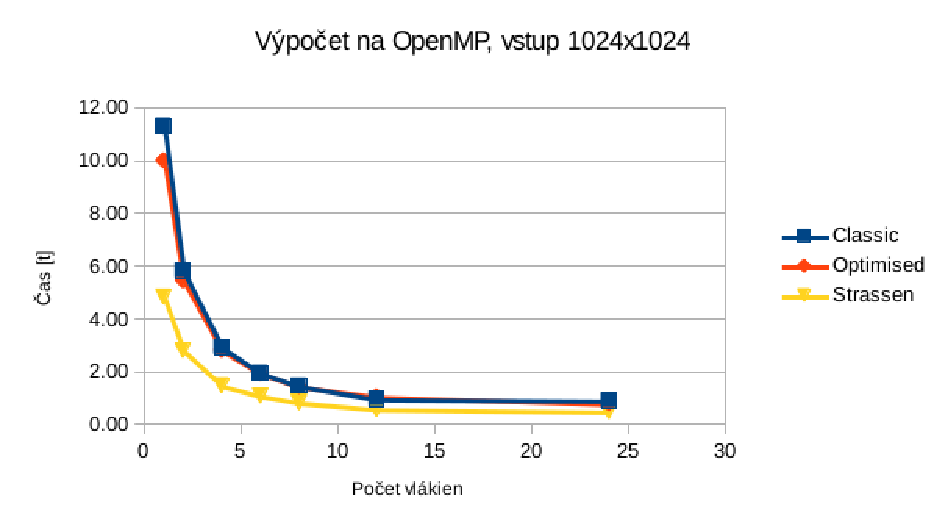
\includegraphics[scale=1]{./images/1024_rychlost.pdf}
	\label{gr:graf1}
\end{figure}

\begin{figure}\centering
	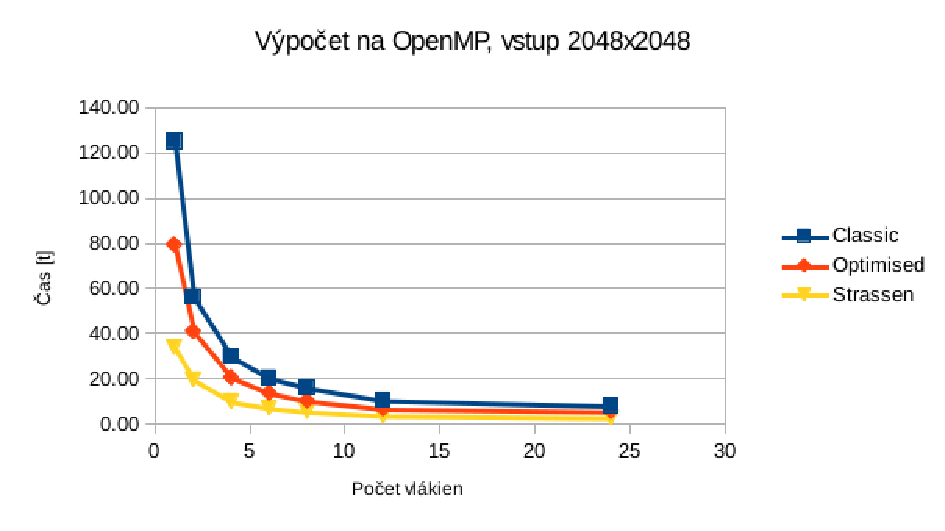
\includegraphics[scale=1]{./images/2048_rychlost.pdf}
	\label{gr:graf2}
\end{figure}  

\begin{figure}\centering
	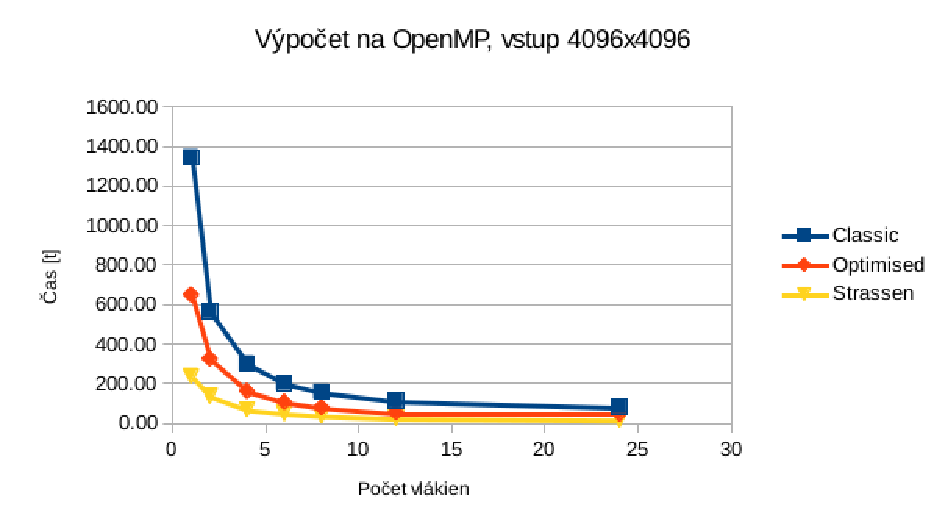
\includegraphics[scale=1]{./images/4096_rychlost.pdf}
	\label{gr:graf3}
\end{figure}  

\begin{figure}\centering
	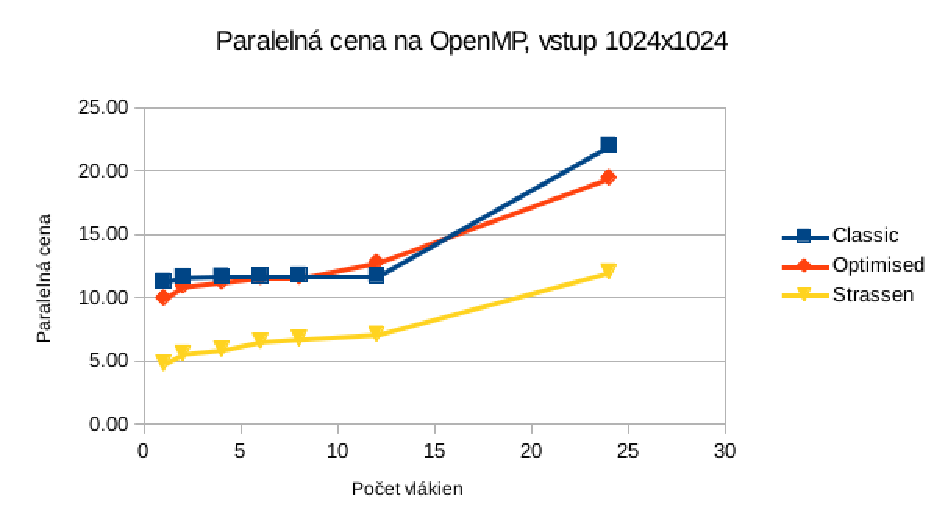
\includegraphics[scale=1]{./images/1024_cena.pdf}
	\label{gr:graf4}
\end{figure}  

\begin{figure}\centering
	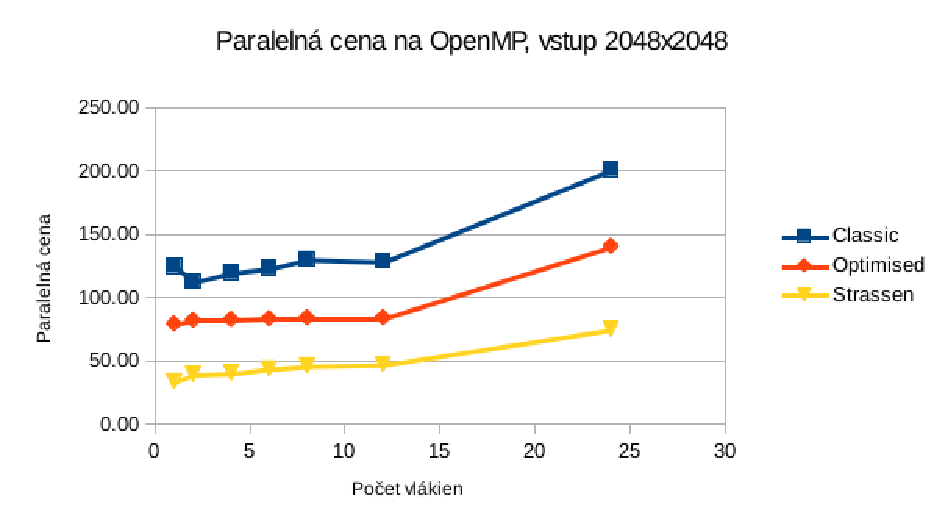
\includegraphics[scale=1]{./images/2048_cena.pdf}
	\label{gr:graf5}
\end{figure}  

\begin{figure}\centering
	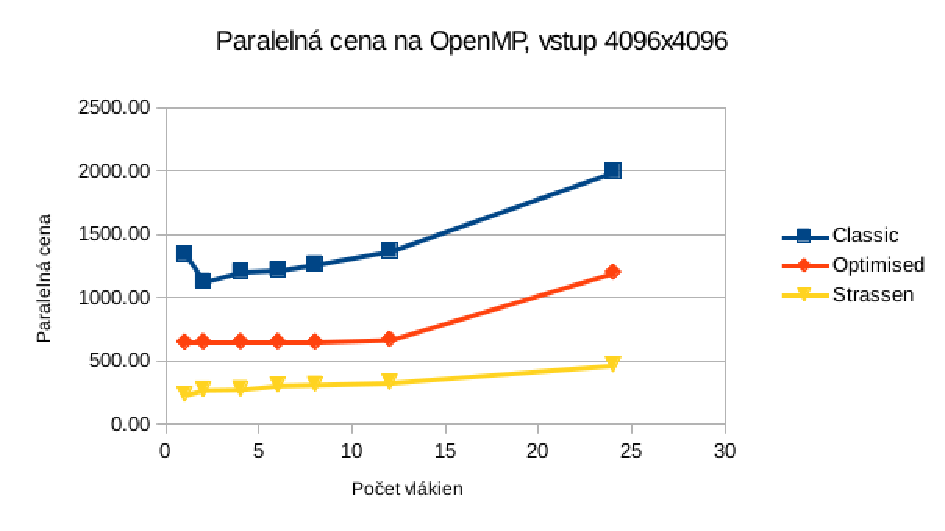
\includegraphics[scale=1]{./images/4096_cena.pdf}
	\label{gr:graf6}
\end{figure}  

Ako môžeme vidieť, pre takmer všetky vlákna (výnimkou je 24 vlákien) a všetky implementácie sme dosiahli približne lineárne zrýchlenie, a teda konštantnú paralelnú cenu. Zvýšenie paralelnej ceny pre 24 vlákien spočíva v tom, že nami použitý hardvér nemal k dispozícii 24 fyzických procesorov, a teda zákonite došlo k prepínaniu kontextu v rámci jedného fyzického procesora. V porovnaní s predmetom BI-PPR, na ktorom sme pracovali s distribuovanou pamätťou, nedošlo k superlineárnemu zrýchleniu. 

Ak by sme porovnávali jednotlivé implementácie medzi sebou, klasický a optimalizovaný algoritmus majú rovnakú asymptotickú zložitosť. Napriek tomu dosahuje optimalizovaná verzia zrýchlenie približne v rozsahu 10 až 50 percent v závislosti od veľkosti vstupu (čím väčší vstup, tým väčšie zrýchlenie). Strassenov algoritmus, ktorého zložitosť je $\mathcal{O}$($n^{2.8074}$), dosahuje v porovnaní s optimalizovanou variantou zrýchlenie približne o 50 percent.

\section{Implementácia na GPU}

Implementáciu na GPU sme vykonali v 2 krokoch. V prvom kroku sme sa sústredili na vytvorenie funkčného riešenia, ktoré pracovalo výlučne s \emph{globálnou GPU pamäťou}. V druhom kroku sme sa časté prístupy do pamäte tohto typu snažili zminimalizovať pomocou \emph{zdieľanej pamäte}, ktorá je súčasťou každého symetrického multiprocesora, a teda bližšie ku koncovým vláknam.

V prvej implementácii sme spúšťali kernel s parametrami \emph{(matrixSize, matrixSize)}, čiže pre každý element výstupnej matice sme spustili 1 vlákno, ktoré v rámci kernelu vykonalo skalárny súčin i-teho riadku matice A s j-tym stĺpcom matice B a výsledok zapísalo do matice C na pozíciu [i][j]. Takto spúšťané riešenie je zároveň limitované hodnotou maximálneho počtu vlákien v rámci jedného bloku, ktorá sa líši v závislosti od Cuda Compute Capabilities (CC). Tento problém sa dá obísť zvýšením počtu blokov a rozdelením do viacerých dimenzií a naopak zmenšením počtu spúšťaných vlákien v 1 bloku tak, aby sa celkový počet spustených vlákien rovnal pôvodnej hodnote druhej mocnine \emph{matrixSize}.

V druhej implmenetácii sme pristúpili k redukcii počtu prístupov do globálnej GPU pamäte. Miesto nej využijeme zdieľanú pamäť - jej problémom je veľkosť rádovo v desiatkach kB, a preto rozdelíme problém násobenia dvoch veľkých matíc na niekoľko násobení menších podmatíc, ktoré sa svojou veľkosťou zmestia do shared memory. Aplikujeme teda podobný princíp ako v prípade optimalizovaného sekvenčného riešenia, v ktorom sme využili loop tiling pre zvýšenie využitia cache pamäte.

Otázkou bolo preto určiť veľkosť submatice. Čim väčšiu veľkosť TILE\textunderscore WIDTH sme volili, tým viac sme využívali shared memory, až sme došli k jej limitom. Tie sa zastavili na hodnote 64, pri ktorej program už nefungoval. Na druhej strane, s narastajúcou veľkosťou TILE\textunderscore WIDTH klesá počet aktívnych blokov, ktoré sa o shared memory v rámci jedného symetrického multiprocesoru navzájom delia. Na základe empirického skúmania sme nakoniec zvolili TILE\textunderscore WIDTH rovnú 16.

\section{Merania na GPU}

Merania sme realizovali na všetkých možných grafických procesoroch na školskom klastri. Výstupom je priemerný čas z trojice meraní pre vstupné matice o veľkosti 256, 512, 1024, 2048, 4096 a 8192. Testy sme realizovali na grafických procesoroch NVIDIA GTX 470, GTX 480, GTX 590 a Tesla K 40. Z výsledkov vidíme, že program bežal najrýchlejšie pre GPU Tesla K40 a naopak najpomalšie pre GeForce GTX 470. Rozdiel medzi týmtito dvomi grafickými akcelerátormi nebol nijako závratný, približne 30 až 40 percent v prospech K 40.

Rozdiel medzi behom na CPU a GPU bol naopak priepastný - pre 24-vláknové CPU nám optimalizovaný algoritmus klasického násobenia bežal nad maticami o veľkosti 4096 približne minútu, zatiaľ čo na GPU bežal nad rovnakým vstupom približne pol sekundy v závislosti od konkrétnej architektúry.

\begin{table}\centering
	\begin{tabularx}{\textwidth}{ | X | X | X | X | X | X | X | }
	  \hline                       
				& \textbf{256} 	& \textbf{512} 	& \textbf{1024} 	& \textbf{2048} 	& \textbf{4096} 	& \textbf{8192} 		\\ \hline
	  \textbf{GTX 470} 	& 0.207 & 1.455 & 11.270& 89.944& 717.77& 5948.61	\\ \hline
	  \textbf{GTX 480} 	& 0.176 & 1.174	& 9.132	& 72.692& 580.81& 4849.28	\\ \hline
	  \textbf{GTX 590} 	& 0.173 & 1.258 & 9.846 & 78.502& 627.67& 5193.220	\\ \hline
	  \textbf{Tesla K40} & 0.140 & 0.936 & 7.509 & 59.764& 476.84& 3787.197  \\ \hline
	\end{tabularx}
\caption{Trvanie behu v ms v prostredí CUDA}
\label{tab2}
\end{table}

\begin{figure}\centering
	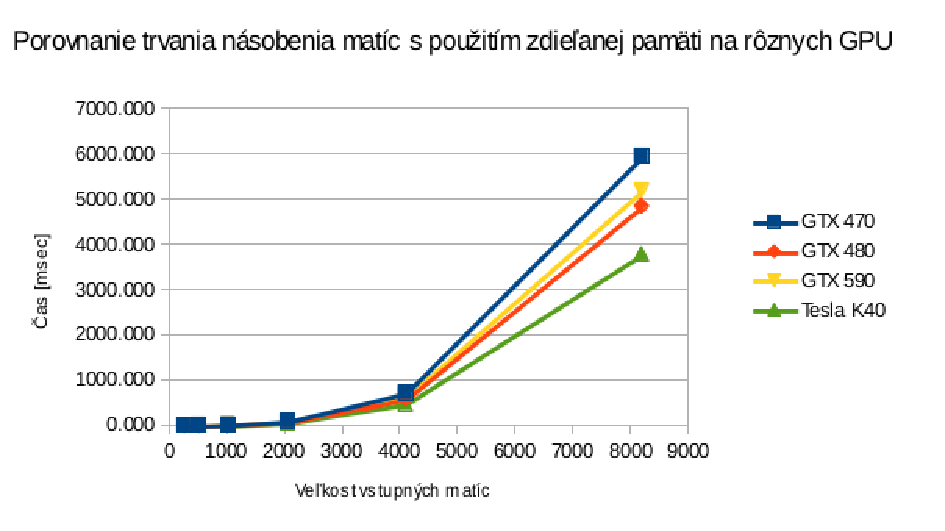
\includegraphics[scale=1]{./images/gpu.pdf}
	\label{gr:graf7}
\end{figure}  

\section{Záver}

Podarilo sa nám implementovať a následne zparalelizovať ako CPU, tak aj GPU verziu násobenia matíc. Program pre CPU sme implementovali v 3 variantách - klasické násobenie, klasické násobenie s loop tilingom a Strassenov algoritmus. Pri následnej paralelizácii v prostredí OpenMP sme dosiahli lineárne zrýchlenie pre všetky tri implementácie. V prostredí GPU sme implementovali výhradne klasický algoritmus, Strassenov algoritmus sme z dôvodu problematickej implementácie rekurzie na GPU vynechali.

Prostredie GPU je mohutne paralelné, pri porovnaní rovnakých vstupných dát (matica 4096), klasický algoritmus s použitím loop tilingu, sme dosiahli 1000-násobné zrýchlenie (10 minút, presne 651.67s na 1-jadrovom CPU vs. 476.84ms na najrýchlejšom GPU, Tesla K40). Na druhej strane, programy v CUDA sú pomerne náročné na implementáciu, zatiaľ čo prostredie OpenMP je svojím high level prístupom veľmi príjemné pre programátora.

\end{document}
